%% 
%%	This is file 'beamer_sample.tex'
%%	according to an MPIDR's PowerPoint template (?)
%%	
%%	by Eric Naujoks
%%
%%	Problems, bugs and comments to 
%%	naujoks@demogr.mpg.de
%%

%%%%%%%%%%%%%%%%%%%%%%%%%%%%%%%%%%
%%	Praelegomena								%%
%%%%%%%%%%%%%%%%%%%%%%%%%%%%%%%%%%
%%	- Make sure that you use utf8-encoding for all your .tex-files!!! (TeXnicCenter since version 2.0)
%%	- TeXnicCenter update: MPIDR intranet > Hard- & Sortfware > Software > Script and text editors > TeXnicCenter

\documentclass[20pt,usenames,dvipsnames]{beamer}

\usepackage[ngerman,english]{babel}
\usepackage{tikz}
 \usepackage{dutchcal}
\usepackage[normalem]{ulem}
\geometry{paperwidth=10in, paperheight=7.5in}
\usepackage{animate}
\usepackage{amsmath,amssymb}

\DeclareRobustCommand{\bbone}{\text{\usefont{U}{bbold}{m}{n}1}}
\DeclareMathOperator{\EX}{\mathbb{E}}% expected value

\usepackage[utf8]{inputenc}

\usepackage[mpidr]{./mpidr/beamerthemeMPIDR}
%\usefonttheme{serif}
%\newcolumntype{C}[1]{>{\centering\let\newline\\\arraybackslash\hspace{0pt}}m{#1}}
%\newcommand*{\QEDA}{\hfill\ensuremath{\blacksquare}}
%% Declaring title and author
%	the institute's logo
%\renewcommand{\mylogo}{\includegraphics[width=4.7in]{mpidr_logo_colour_en}}
\usepackage{color}
\definecolor{mygray}{rgb}{0.8,0.8,0.8}
\definecolor{mygray2}{rgb}{0.5,0.5,0.5}
\definecolor{yellow}{rgb}{1,1,0}

\defbeamertemplate{description item}{align left}{\insertdescriptionitem\hfill}
%%	should be the very last package to be loaded
\usepackage{hyperref}

%%%%%%%%%%%%%%%%%%%%%%%%%%%%%%%%%%
%%	Beginning of the document		%%
%%%%%%%%%%%%%%%%%%%%%%%%%%%%%%%%%%
\begin{document}

%%	titlepage - fixed frame:
%%	========================

% \begin{frame}
% 	\titlepage
% \end{frame}
\begin{frame}[plain]
	%\titlepage
	\vspace{-3cm}
 \centerline{\includegraphics[scale=.165]{beamerstrip3.png}}

	\huge
	\vspace{1em}
	
	Decomposition perspectives on distributions of episode duration \\
	\vspace{1em}
	\large 
	Tim Riffe \pause | HT C. Dudel \& D. Schneider
\end{frame}
%-------------------

\begin{frame}[plain]
\Large
\centering
 Some motivating observations:\vspace{2em}
 \begin{enumerate}[<+->]
 \item Health \emph{inequality} is multidimensional: episode duration important? 
 \item Dudel's expression for average episode count \& duration: how about distributions?
 \end{enumerate}
\end{frame}

\begin{frame}[plain]
\Large
A common sight:\vspace{-1em}
\begin{center}
\includegraphics[scale=.9]{Figures/Expectancies.pdf}
\end{center}
\end{frame}

\begin{frame}[plain]
\Large
\centering
 Motivating questions:\vspace{2em}
 \begin{enumerate}[<+->]
 \item How do state expectancies break down by episode duration?
 \item What is the age pattern of episode duration?
 \item Extra 1: how much of a state expectancy is from terminal episodes?
 \item Extra 2: how do transition probabilities determine episode distributions?
 \end{enumerate}
\end{frame}
% probabilities of starting a new episode (left anchor)
% ---------------------
\begin{frame}[plain]
\Large
\centering
 Probability of a new episode $\epsilon$ in state $s$ starting at age $x$:\vspace{2em}
 \begin{equation}
 \epsilon^{s,new}(x) = \pi^{-s}(x) \cdot p^{\rightarrow s}(x)
 \end{equation}
 \begin{itemize}
 \item $\epsilon^{s,new}$ new episode of $s$
 \item $\pi^{-s}$ prevalence of not being in $s$
 \item $p^{\rightarrow s}$ probaility of transition to $s$
 \end{itemize}
\end{frame}

% ---------------------
\begin{frame}[plain]
\Large
\begin{itemize}[<+->]
\item Let $\textbf{E}^s$ be a matrix with $\epsilon^{s,new}$ in the diagonal
\item Let $\textbf{U}^s$ be a matrix with $p^{s\rightarrow s}$ in the subdiagonal
\item Let $\textbf{N}^s = \left( \textbf{I} - \textbf{U}^s \right)^{-1}$ 
\item Then the conditional elapsed time spent in $s$: $\mathbcal{E}^s = \textbf{N}^s \textbf{E}^s$
\item $\EX(s,x) = \textbf{e}' \mathbcal{E}^s \textbf{e} + \textcolor{mygray2}{p^s(x) \sum_{t=x}^\omega \prod_{i=t}^\omega p^{s\rightarrow s}(i)}$ 
\item The matrix $\mathbcal{E}^s$ is a decomposition of  $\EX(s)$ by age and elapsed time in $s$
\end{itemize}

\end{frame}
% ---------------------


%----------------------
\begin{frame}[plain]
\Large
\begin{center}
An illustration \vspace{2em}
\pause
\begin{itemize}[<+->]
  \item Recycle transition probabilities from \normalsize{Riffe, Mehta,
  Schneider \& Myrskyl\"a (in progress)} (HRS data).
  \item 3 states: 0 ADLs, 1+ ADLs, dead.
  \item ages 50+, 2-year age groups
\end{itemize}
\end{center}
\end{frame}


\begin{frame}[plain]
\Large
Transitions for 2006 females (all edu):\vspace{-1em}
\begin{center}
\includegraphics[scale=1]{Figures/TransitionsInk.pdf}
\end{center}
\end{frame}

\begin{frame}[plain]
\Large
Prevalence for 2006 females (all edu):\vspace{-1em}
\begin{center}
\includegraphics[scale=1]{Figures/PrevalenceInk.pdf}
\end{center}
\end{frame}

\begin{frame}[plain]
\Large
Prevalence disabled 2006 females (all edu):\vspace{-1em}
\begin{center}
\includegraphics[scale=1]{Figures/PrevalenceDisR.pdf}
\end{center}
\end{frame}

\begin{frame}[plain]
\Large
Disability decomposed 2006 females (all edu):\vspace{-1em}
\begin{center}
\includegraphics[scale=1]{Figures/DisByDur.pdf}
\end{center}
\end{frame}

\begin{frame}[plain]
\Large
Disability decomposed 2006 females (all edu):\vspace{-1em}
\begin{center}
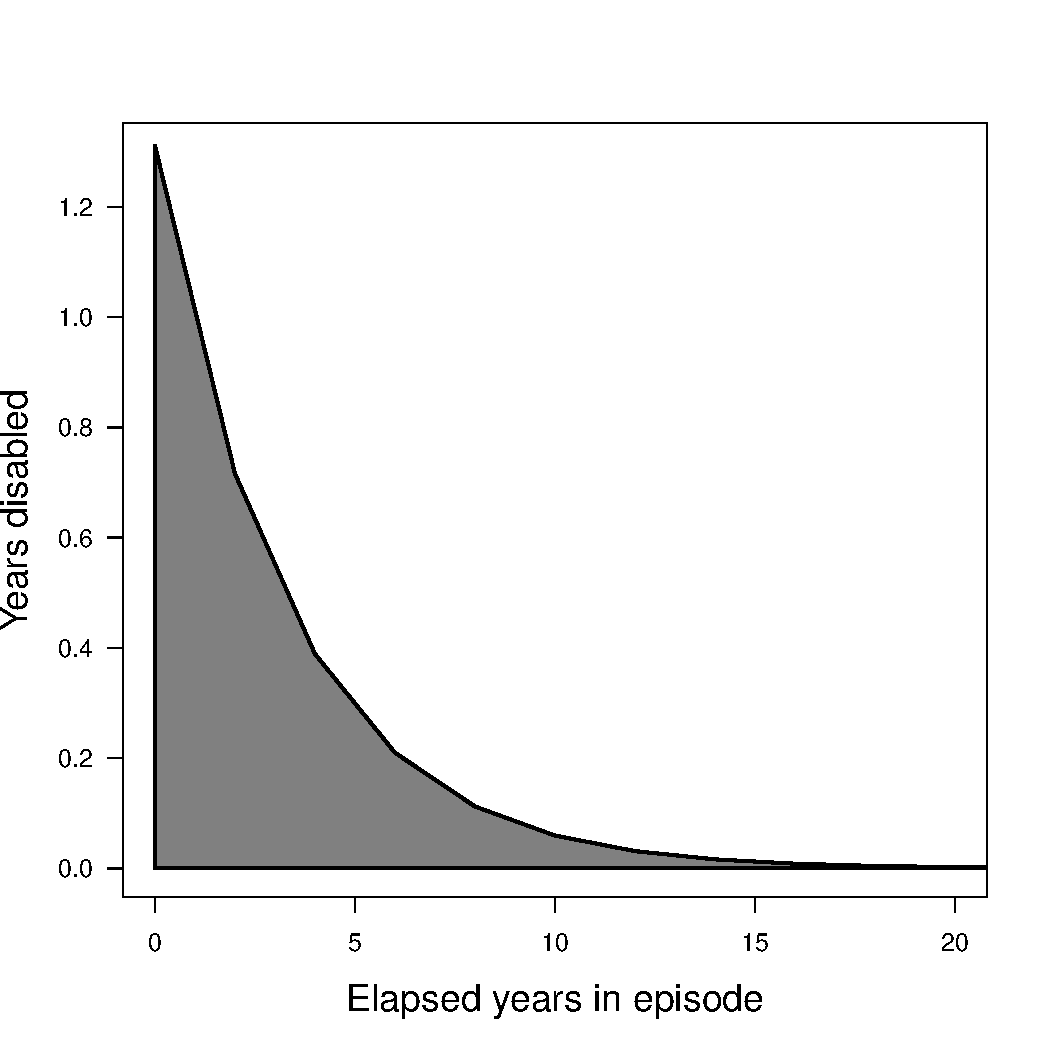
\includegraphics[scale=1]{Figures/DisElapsed.pdf}
\end{center}
\end{frame}

\begin{frame}[plain]
\Large
Disability decomposed 2006 females (all edu):\vspace{-1em}
\begin{center}
\includegraphics[scale=1]{Figures/DisTotalDur.pdf}
\end{center}
\end{frame}

\begin{frame}[plain]
\Large
\centering
Are the contents of such decompositions relevant to health inequality?
\end{frame}

\begin{frame}[plain]
\Large
\centering
Extra 1: terminal vs other states.

\pause
Deaths by age and elapsed time of terminated episode

$\textbf{D}^s = diag(\textbf{p}^{s\rightarrow \dagger}) \mathbcal{E}^s $

\end{frame}

\begin{frame}[plain]
\Large
\vspace{1em}
\begin{center}
Proportion of DLE composed of terminal episodes, by sex and education:\vspace{-1em}
\includegraphics[scale=.9]{Figures/PropTerminalEdu.pdf}
\end{center}
\end{frame}

\begin{frame}[plain]
\Large
\begin{center}
Extra 2: everything is a function of transition probabilities

\vspace{1em}
\pause
Use general decomposition method, such as Horiuchi et. al. (2008) in \texttt{R} package \texttt{DemoDecomp}
\end{center}
\end{frame}


\usebackgroundtemplate{%
  \includegraphics[width=\paperwidth,height=\paperheight]{willian-justen-de-vasconcellos-595793-unsplash.jpg}} 
\begin{frame}[plain]
\Large
\centering
Episode decomposition and healthy inequality\\ What are your thoughts?\\ \vspace{1em}Thanks!
\tiny
\flushright
\vspace{13cm}
   Photo by Willian Justen de Vasconcellos
\end{frame}
%%%%%%%%%%%%%%%%%%%%%%%%%%%%%%%%%%
%%	End of the document			%%
%%%%%%%%%%%%%%%%%%%%%%%%%%%%%%%%%%
\end{document}






